\documentclass[12pt,reqno]{article}
\usepackage[dutch]{babel}
\usepackage[margin=1.2in]{geometry}
\usepackage{amsmath}
\usepackage{amssymb}
\usepackage{color}
\usepackage{makeidx}
\usepackage{natbib}
\usepackage{tikz}
\usepackage{tkz-euclide}
\usepackage{url}

\title{\textbf{Congruente getallen}\\
		\small{eerste versie studentencheck}}
\author{
	\begin{tabular}{ l l }
		Lotte Bruijnen, & 4297652 \\
		Daan van Laar, & 5518741 \\
		Suzanne Vincken, & 4273338
	\end{tabular}\\
	Onder begeleiding van: Carel Faber, UU
}
\date{10-12-2015}

\newcommand*{\NN}{\ensuremath{\mathbb{N}}}
\newcommand*{\ZZ}{\ensuremath{\mathbb{Z}}}
\newcommand*{\QQ}{\ensuremath{\mathbb{Q}}}
\newcommand*{\RR}{\ensuremath{\mathbb{R}}}
\newcommand*{\CC}{\ensuremath{\mathbb{C}}}
\newcommand*{\QED}{\hfill\ensuremath{\blacksquare}}

\begin{document}
	
	\maketitle
	%\thispagestyle{empty}
	%\pagestyle{empty}
	\allowdisplaybreaks
	
	\section{Inleiding}
	We gaan het hebben over congruente getallen. Eerst vindt u een begrippenlijst, zodat u de betekenis van veelvoorkomende begrippen altijd op kan zoeken. Daarna wordt er uitgelegd wat congruente getallen zijn en wat dit te maken heeft met Pythagorese drietallen. We gaan kijken hoe we alle congruente getallen kunnen vinden en daarna zullen we ook kijken naar een aantal belangrijke stellingen.
	
	
	\section{Begrippen}
	\begin{tabular}{ p{4,6cm} p{10cm} }
		\textbf{Kwadraatvrij}: \cite{Beukers} & Een kwadraatvrij getal is een getal dat niet deelbaar is door een kwadraat groter dan $1$. Waarbij een kwadraat een getal $k\in\NN$ zodat $\sqrt{k}\in\NN$. \\
		\textbf{Primitieve congruente getallen}: & Een kwadraatvrij congruent getal. \\
		\textbf{begrip}: & uitleg \\
		\textbf{begrip}: & uitleg
	\end{tabular}
	
	\section{Congruente getallen en Pythagorese drietallen}
	\section{Daan}
	
	Stel, $\exists \delta \in \QQ$. Een getal $n \in \NN$ heet een congruent getal als $\delta^2 - n$, $\delta^2$ en $\delta^2 + n$ kwadraten zijn in \QQ. Dat wil zeggen, $\delta^2 - n$, $\delta^2$ en $\delta^2 + n$ zijn te schrijven als $\left(\dfrac{p}{q}\right)^2$ met $p, q \in \NN$\\
	Een getal dat aan deze definitie voldoet is het getal 5, dus we stellen $n = 5$. We nemen $\delta = \dfrac{41}{12}$. Dan is $\delta^2 = \left( \dfrac{41}{12} \right)^2, \delta^2 - n = \dfrac{1681}{144} - 5 = \dfrac{961}{144} = \left( \dfrac{31}{12}\right)^2	en  \delta^2 + n = \dfrac{1681}{144} + 5 = \dfrac{2401}{144} = \left( \dfrac{48}{12}\right)^2$
	
	%\section{Daan}
	
	
	\section{voorbeelden}
	Het kleinste congruente getal is $5$. Dat is de driehoek met de volgende zijden:
	\begin{figure*}[h!]
		\centering
		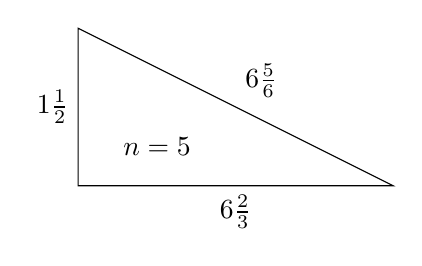
\begin{tikzpicture}[xscale=4, yscale=2]
		\coordinate (O) at (0,0);
		\coordinate (A) at (1,0);
		\coordinate (B) at (0,1);
		\coordinate (M) at (0.25, 0.25);
		\draw (O) -- node[auto,swap]{$6\frac{2}{3}$} 
		(A) -- node[auto,swap]{$6\frac{5}{6}$}
		(B) -- node[auto,swap]{$1\frac{1}{2}$}cycle;
		\draw (M) node[auto]{$n=5$};
		\end{tikzpicture}
	\end{figure*}\\
	Het kleinste congruente getal met zijden uit $\NN$ is $6$. Dat is de driehoek met de volgende zijden:
	\begin{figure*}[h!]
		\centering
		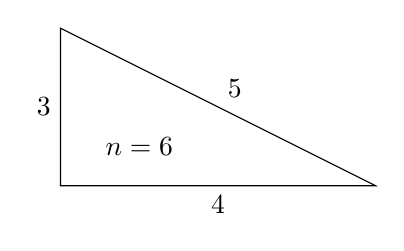
\begin{tikzpicture}[xscale=4, yscale=2]
		\coordinate (O) at (0,0);
		\coordinate (A) at (1,0);
		\coordinate (B) at (0,1);
		\coordinate (M) at (0.25, 0.25);
		\draw (O) -- node[auto,swap]{$4$} 
		(A) -- node[auto,swap]{$5$}
		(B) -- node[auto,swap]{$3$}cycle;
		\draw (M) node[auto]{$n=6$};
		\end{tikzpicture}
	\end{figure*}\\
	Dit is de driehoek met oppervlakte $157$: \cite{Koblitz}[p.5]
	\begin{figure*}[h!]
		\centering
		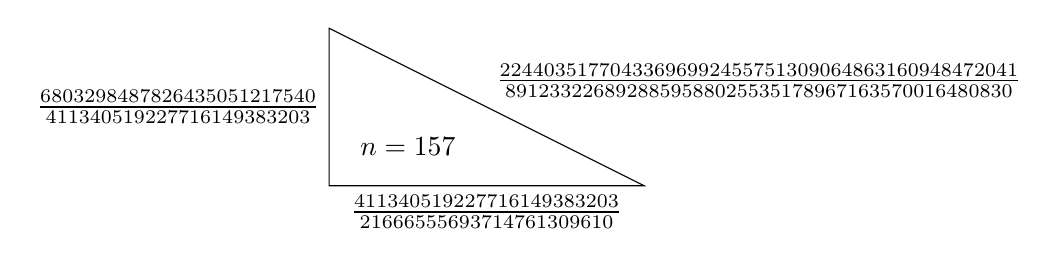
\begin{tikzpicture}[xscale=4, yscale=2]
		\coordinate (O) at (0,0);
		\coordinate (A) at (1,0);
		\coordinate (B) at (0,1);
		\coordinate (M) at (0.25, 0.25);
		\draw (O) -- node[auto,swap]{$\frac{411340519227716149383203}{21666555693714761309610}$} 
		(A) -- node[auto,swap]{$\frac{22440351770433696992455751309064863160948472041}{8912332268928859588025535178967163570016480830}$}
		(B) -- node[auto,swap]{$\frac{6803298487826435051217540}{411340519227716149383203}$}cycle;
		\draw (M) node[auto]{$n=157$};
		\end{tikzpicture}
	\end{figure*}
	
	
	\section{Congruente getallen vinden}
	Het volgende komt uit \cite{Koblitz}[p.3-4].\\
	We weten nu dat een een congruent getal $n$ een geheel getal is als oppervlakte van een driehoek met rationale zijden. Als we nu willen kijken welke $n'\in\NN$ congruente getallen zijn, moeten we heel $\NN$ door. Dit is niet te doen. Daarom willen we het aantal mogelijke waardes van $n'$ beperken. We doen het volgende:\\
	Neem een getal $r\in\QQ$ en zeg $r$ is congruent. Dan zijn $x,y,z\in\QQ$ de zijden van de rechthoekige driehoek met oppervlakte $r$. We kunnen nu voor elke $r\neq0$ een $s\in\QQ$ vinden zodat $s^2r$ een kwadraatvrij natuurlijk getal is.
	\begin{itemize}
		\item[] \underline{Bewijs}: We weten $r\in\QQ$, dus $r$ is te schrijven als: $r=\frac{p}{q}$. Neem nu een $s\in\QQ$ zodat $s^2$ deelbaar is door $q$. {\color{red}Nu geldt dat $s^2r$ een kwadraatvrij getal.}\QED
	\end{itemize}
	We weten nu dat $s^2r$ een kwaadraatvrij getal is. En we doen het volgende: neem de driehoek met zijden $sx,sy,sz$. De oppervlakte van deze driehoek is $s^2r$. We kunnen nu zonder verlies van algemeenheid zeggen dat $s^2r=n$. We kunnen dus ook aannemen dat $n$ een congruent kwadraatvrij natuurlijk getal, oftewel een primitief congruent getal, is. We weten dan ook dat $s^2n$, met $s^2\in\QQ$, een congruent getal is.  \\
	
	We hebben hierboven gezien dat we de mogelijke waardes van $n'$ hebben beperkt, omdat $n'$ nu een kwadraatvrij getal is. Dus we kunnen nu al een stuk sneller door $\NN$ om te kijken welke getallen $n'\in\NN$ congruent zijn. Sterker nog: er betstaat een algoritme die voor elke $n'$ checkt of er een Pythagorees drietal bestaat zodat $n'$ de oppervlakte is van deze driehoek (dus $n'=n$). Als $n'$ congruent is, zet het algoritme deze in een lijst. Het probleem hierbij is dat we niet weten hoe lang we moeten zoeken naar een Pythagorees drietal die bij $n'$ past. Dus als $n'$ niet in de lijst staat, weten we niet of (1) $n'$ geen congruent getal is of (2) dat het zoeken te lang duurde en het zoeken is afgebroken. Wat we dus eigenlijk willen is een gesloten formule vinden, zodat we makkelijk kunnen checken of $n'$ een congruent getal is of niet.\\
	
	Elliptische krommen zijn krommen die voldoen aan de vergelijking $y^2=x^3-n^2x$.
	
	
	\section{Stellingen}
	\newtheorem{Tunnell}{Theorem}
	\begin{Tunnell}
		\cite{Koblitz}[p.212] (Tunnell, 1983) If $n$ is a squarefree and odd (respectively, even) positive integer ans $n$ is the area of a right triangle with rational sides, then
		\begin{align}
		\#\{x,y,z\in\ZZ|n=2x^2+y^2+32z^2\} = \frac{1}{2}\#\{x,y,z\in\ZZ|n=2x^2+y^2+8z^2\}\\
		\notag \text{(respectively, } \\
		\#\{x,y,z\in\ZZ|\frac{n}{2}=4x^2+y^2+32z^2\} = \frac{1}{2}\#\{x,y,z\in\ZZ|\frac{n}{2}=4x^2+y^2+8z^2\})
		\end{align}
		If the weak Birch-Swinnerton-Dyer conjecture is true for the elliptic curves $E_n:y^2=x^3-n^2x$, then, conversely, these equalities imply that $n$ is a congruent number.
	\end{Tunnell}
	
	\newtheorem{CG}{Defenitie}
	\begin{CG}
		\cite{Oort}[p.3] Een positief geheel getal $N$ heet een congruent getal als er een rechthoekige driehoek bestaat met lengtes van zijden in $\QQ_{>0}$ en met oppervlak gelijk aan $N\in\ZZ$. Noem de lengtes van de zijden $a,b,c\in\QQ$; met behulp van de stelling van Pythagoras zien we:
		\begin{figure*}[h!]
			\centering
		\begin{tikzpicture}[xscale=6, yscale=3]
		\coordinate (O) at (0,0);
		\coordinate (A) at (1,0);
		\coordinate (B) at (0,1);
		\draw (O) -- node[auto,swap]{$\alpha$} 
		      (A) -- node[auto,swap]{$\gamma$}
		      (B) -- node[auto,swap]{$\beta$}cycle;
		\coordinate (M) at (1.5, 0.5);
		\draw (M) node[auto]{$\alpha\cdot\beta/2=N$};
		\coordinate (N) at (1.5, 0.25);
		\draw (N) node[auto]{$\alpha^2+\beta^2=\gamma^2$};
		\end{tikzpicture}
		\end{figure*}\\
	\end{CG}
	
	
	\bibliographystyle{plain}
	\bibliography{bib}
\end{document}